\documentclass{beamer}

\usepackage{upquote}
\usepackage{color}
\usepackage{alltt}
\usepackage{graphicx}
\usepackage{listings}
\usepackage{multicol}
\lstset{ %
  basicstyle=\Tiny\ttfamily\color{blue}, %
  frame=single, %
  includerangemarker = false, %
  title = \tiny\ttfamily\color{blue}\emph{Interactive Stata Example}, %
  captionpos = t, %
  %xleftmargin=-0.6cm, %
  rangeprefix=*@*%, %
  %belowcaptionskip = -0.08in, %
  %label={bla}
}

\usetheme{Boadilla}

%\usecolortheme{orchid}
%\usecolortheme{beaver}
%\setbeamercolor{item projected}{fg=black,bg=white}
\usecolortheme{beaver}
\setbeamertemplate{itemize subitem}[triangle]
\setbeamercolor{item projected}{fg=darkred, bg=lightgray}
\setbeamercolor{subitem projected}{fg=darkred}
\setbeamercolor{local structure}{fg=darkred}


\usefonttheme{professionalfonts}

%\usepackage{verbatim}
%{\catcode`\`=13 \g@addto@macro\@verbatim{\chardef`=18 }}

\title{MPP-C6: Statistics II}
\subtitle{Programming with Stata}
\author{Max Callaghan}
\institute[HSoG]{Hertie School of Governance}
\titlegraphic{
\includegraphics[width=2cm]{HSOG_logo.png}}
\date{?? February 2015}


\begin{document}

\frame{\titlepage}

\begin{frame}
  \frametitle{Outline}
  \begin{itemize}
    \item Why Program?
    \item Reproducible Research
    \item Programming in Stata to accomplish difficult tasks and simplify repetitive tasks
  \end{itemize}
\end{frame}

\begin{frame}
  \frametitle{Why Program?}
  \begin{itemize}
    \item Computers can perform calculations faster and more accurately than humans
    \item When a task is difficult or repetitive, if often makes sense to instruct the computer to do it
    \item When those instructions are written down, we and others can see exactly what has been done
    \begin{itemize}
      \item It's easier to repeat the work
      \item It's easier to spot errors
      \item It's easier to repeat the work, changing just one detail, without doing every subsequent step again.
    \end{itemize}
  \end{itemize}
\end{frame}

\begin{frame}
  \frametitle{Reproducible Research}
  \begin{itemize}
    \item ``The standard of reproducibility calls for the data and the computer code used to analyse the data to be made available to others" \cite{Peng}
    \item Literate programming ties together data, code and the actual research output, enhancing reproducibility
  \end{itemize}
\end{frame}

\begin{frame}
  \frametitle{Reproducible Research}
  \frametitle{Reproducible Research with Stata}
  \begin{itemize}
    \item What do we already do that helps to keep our research reproducible?
    \item How do we ensure that what's in our research output reflects the calculations we report making?
  \end{itemize}
\end{frame}

\begin{frame}
  \frametitle{Reproducible Research}
  \frametitle{Reproducible Research with Stata}
  \begin{itemize}
    \item The ideal for perfect reproducibility would be to have a single document that contains instructions for performing calculations as well as for producing the research output we present.
    \item This is not possible in Stata without \LaTeX\ but we can at least make the way we include Stata output in Word documents more systematic
  \end{itemize}
\end{frame}

\begin{frame}
  \frametitle{Reproducible Research}
  \frametitle{Reproducible Research with Stata}
  [Include instructions to do this, with a simple example of output that changes to reflect a change in a do file]
\end{frame}

\begin{frame}
  \frametitle{Programming with Stata}
  %\framesubtitle{Stata Refresher}
  \framesubtitle{Outline}
  \begin{itemize}
    \item Stata basics
    \item Directory structure
    \item Reading data
    \item Transforming and processing data
    \item Presenting results with Stata
  \end{itemize}
\end{frame}

\begin{frame}
  \frametitle{Programming with Stata}
  \frametitle{Stata Basics}
  %\framesubtitle{Outline}
  \begin{itemize}
    \item Pointing and clicking is fine for exploring data
    \item The command line is fine for trying out commands
    \item Anything you want to be able to reproduce, you should put in the do file
  \end{itemize}
\end{frame}

\begin{frame}[fragile]
  \frametitle{Programming with Stata}
  \frametitle{Stata Basics}
  \framesubtitle{Writing a good do file}
  A good do file should be readable by humans as well as computers.
  \begin{itemize}
    \item Use comments to explain what each line is doing
    \item Empty lines are free, space makes your code easier to read
    \item Use meaningful names when you create them, and write them consistently (variable\_name, variableName or VariableName)
    \item Follow indentation conventions e.g.
    \begin{verbatim}
forvalues i in 1/5 {
  display `i'
}
    \end{verbatim}
  \end{itemize}
\end{frame}

\begin{frame}[fragile]
  \frametitle{Programming with Stata}
  \frametitle{Stata Basics}
  \framesubtitle{Understanding Stata Commands}
  Stata commands are preprogrammed functions that take information we give to them, do something with the information, then output something. We pass information to commands with \textit{arguments} and \textit{options}.
  
  If you are not sure how to use a command you can get help by typing "help" and then the name of the command. For example,
  \begin{verbatim} help regress \end{verbatim}
  will take you to the regress command's \href{http://www.stata.com/manuals13/rregress.pdf}{manual}
\end{frame}

\begin{frame}
  \frametitle{Programming with Stata}
  \frametitle{Stata Basics}
  \framesubtitle{Reading the Stata manual}
  The Syntax \texttt{\underline{reg}ress} \textit{\textcolor{blue}{depvar [indepvars] [if] [in] [weight]} [,options]} describes the basic use of the command
  \begin{itemize}
    \item Pay attention to the order of the arguments. This is how Stata knows which arguments are which
    \item Items in square brackets are optional
    \item Options come after a comma. Possible options are described in the help file
    \item You don't always need to set a lot of options, but you should pay atention to what the defaults are
  \end{itemize}
  If you don't know the command you want to use, you will have try and describe your problem to google.
\end{frame}

\begin{frame}
  \frametitle{Directory Structure}
  %\framesubtitle{Directory Structure}
  File paths tell the computer where to read and write information. They differ between Windows and Mac/Linux. (\textbackslash or /)
  \begin{itemize}
    \item Absolute paths start from the top of the tree and specify each subdirectory until the file e.g. "C:bla\textbackslash bla\textbackslash data.dta" (or "/bla/bla/data.dta", or even "http://bla.com/data.dta")
    \item Relative paths start from the current working directory; use ../ or ..\textbackslash to move to the directory above the current one
  \end{itemize}
\end{frame}

\begin{frame}
  \frametitle{Directory Structure}
  \framesubtitle{}
  If you refer to more than one resource, it makes sense to set the working directory at the top of your do file and use relative paths. You'll want to think about how you structure your directory so that you can access items easily.
  \begin{itemize}
    \item If your do file produces output, think about where you want to save it so that you can access it automatically with another program
    \item This also allows you to change computers easily. Dropbox is an easy way to carry entire directories between computers. \href{https://desktop.github.com/}{Git/Github} is even better as it incorporates version control.
  \end{itemize}
\end{frame}

\begin{frame}
  \frametitle{Reading Data}
  \framesubtitle{}
Data doesn't always come in nicely formatted dta files. Sometimes you have a data source or sources in files that aren't set up for stata to read. You often have to do a bit of work to get things into the format you want: the more of that work is recorded the better.


\end{frame}

\begin{frame}
  \frametitle{Reading Data}
  \framesubtitle{}
Some things to pay attention to when reading data
  \begin{itemize}
    \item Keep an original copy of the data exactly as you found it, if you make changes, save to a new name
    \item Try and make changes with Stata in your do file. If you have to change in Excel, write down what you did
    \item Check the data has been imported properly before you use it
	\begin{itemize}
	    \item You may need to specify what character signifies missing values in your data 
	    \item You might need to specify the delimiter in csv or txt files
	    \item 
	\end{itemize}
    \item 

  \end{itemize}
\end{frame}

\begin{frame}
  \frametitle{Data types}
  \framesubtitle{}
Stata stores data in various different data types. Each variable can only be one data type. Some operations can only be done on data of certain types
  \begin{itemize}
    \item Numeric data can be stored in various degrees of precision: check -help data types- for more information
    \item Anything with non-numeric characters will be saved as a string (text)
  \end{itemize}

It's easy for data to arrive in the wrong format when we read from other sources.


We can use -tostring- and -destring- to convert between string and numeric data, as well as -encode- to create a numeric variable out of non-numeric string data.
\end{frame}

\begin{frame}[fragile]
  \frametitle{Processing Data}
  %\framesubtitle{Macros}
  \begin{itemize}
    \item -keep- and -drop- can remove observations we don't want
    \item -gen- and -egen- create new variables
    \item -replace- can change the values of a variable
  \end{itemize}
All can be applied selectively with if conditions

\end{frame}

\begin{frame}[fragile]
  \frametitle{Programming with Stata}
  \framesubtitle{Macros}
  Stata already helps us to perform calculations quickly, but we can speed up how we interact with Stata by using some simple programming to avoid repetition.  The most simple concept is storing something as a macro.
  \begin{itemize}
    \item Macros can tie a name to some text 
    \item \verb|local controls age gender incCat| ties the word "controls" to ``age gender inc\_cat''
    \item Now, everytime we type  \verb|`controls'|, stata understands ``age gender inc\_cat'' (note the backtick, which is under the tilde)
    \item If we type ``age gender inc\_cat'' a lot, then we save ourselves time by defining it once and referring to the definition the other times
    \item This also reduces the risk of errors. Why?
  \end{itemize}
\end{frame}

\begin{frame}[fragile]
  \frametitle{Programming with Stata}
  \framesubtitle{Loops}
  Loops can speed up our work by repeating tasks while changing one thing. 
  \begin{verbatim}
foreach control of local controls {
  display "`control'"
}
  \end{verbatim}
  Will loop through our list of controls, and perform the command -display- on each of them.

\smallskip

As with macros, we initialise the iterator without quotes, and insert its value into our commands using the backtick and single quote
\end{frame}

\begin{frame}[fragile]
  \frametitle{Programming with Stata}
  \framesubtitle{Loops}

 We can perform any commands we want inside the loop, including using more loops and if conditions.
What would be the outcome of this loop?
  \begin{verbatim}
forvalues i = 1/20 {
  if mod(`i',2)==0 {
    di "`i' is even"
  } else {
    di "`i' is odd"
  }
}
  \end{verbatim}

\end{frame}

\begin{frame}[fragile]
  \frametitle{Programming with Stata}
  \framesubtitle{Exercise - are you smarter than a 10 year old?}

\textbf{\Large Fizz-Buzz}
\medskip

Count up to 100, replacing any number divisible by three with the word "fizz", and any number divisible by five with the word "buzz", and any number divisible by both with "fizz-buzz".

\medskip

Can you write a loop in Stata that plays fizzbuzz correctly? (2 minutes)
\end{frame}


%Explain how this fits into the logic of programming - repeating a process, evaluating conditions - more accurate
\begin{frame}[fragile]
  \frametitle{Programming with Stata}
  \framesubtitle{Exercise - are you smarter than a 10 year old?}
 \begin{verbatim}
forvalues i = 1/100 {
  if mod(`i',3)==0 & mod(`i',5)==0{
    di "fizzbuzz"
  } 
  else if mod(`i',5)==0{
    di "buzz"
  }
  else if mod(`i',3)==0{
    di "fizz"
  }
  else {
    di "`i'"
  }
}
  \end{verbatim}
\end{frame}

\begin{frame}[fragile]
  \frametitle{Programming with Stata}
  \framesubtitle{The -by- command}
Another way to repeat calcuations is using -by-.

\medskip

-by- temporarily splits your data into subsets for every value of a variable and performs the command on that subset.

\medskip

To use the by command you need to -sort- your data
\end{frame}

\begin{frame}[fragile]
  \frametitle{Programming with Stata}
  \framesubtitle{The -by- command}

\lstinputlisting[linerange={lstart-lend}]{../../stata/logs/byreg.log}

\end{frame}

%%%%%%%%%%%%%%%%%%%%%%%%%%%%%%%%%%%%%%%%%%%%%% Practical application 1st section


\begin{frame}
  \frametitle{Example 1}
  \framesubtitle{Reading Data}
Now we want to apply some of this to a real world example.

\medskip

We've found an interesting data source on the web \href{http://data.london.gov.uk/dataset/metropolitan-police-service-recorded-crime-figures-and-associated-data/resource/e831234d-2bde-4fff-8ab8-7e2e70f0677a}{(link)}.  

\medskip

It's an excel sheet containing various crime related data in different boroughs over different time periods.

\medskip

There's an interesting panel dataset in there but we have to work to get it.

\end{frame}

\begin{frame}
  \frametitle{Example 1}
  \framesubtitle{Reading Data}

We start by copying the data it onto our computer and use -import excel- to read into stata the sheet "Fear of Crime-Borough".
\lstinputlisting[linerange={lstart-lend}]{../../stata/logs/foCrime_import.log}

\end{frame}




%%%%%%%%%%%%%%%%% do this on the board
\begin{frame}
  \frametitle{Example 1}
  \framesubtitle{Cleaning data}
Sometimes data is input incorrectly - in this case we have 2 records for September 2008. Since we don't know which is correct, it's probably safer to remove them both.

\lstinputlisting[linerange={lstart-lend}]{../../stata/logs/foCrime_clean.log}

For each value of the date, we set dup to 1 if the number of observations (\_N) with that value is 1, otherwise we set it to the number of each observation (\_n)

\end{frame}


\begin{frame}
  \frametitle{Example 1}
  \framesubtitle{Transforming data}
In stata, columns are called variables and rows are observations. We don't always receive data like that.

\smallskip

How would you reformat this data? What variables do we have?

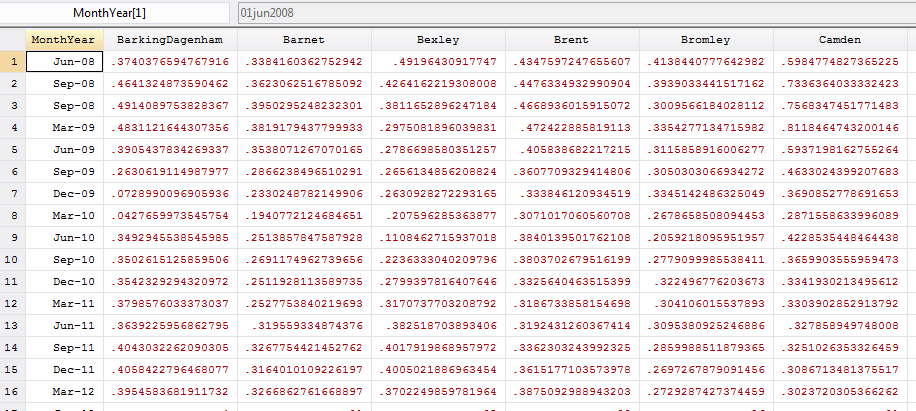
\includegraphics[width=5in]{data.PNG}
\end{frame}


\begin{frame}
  \frametitle{Example 1}
  \framesubtitle{Transforming data}
Our data is too wide: we can use the -reshape- command to switch between ``wide" and ``long" formats. First we need to give the borough coloums a common prefix, then we can tell reshape to create a new variable. While we're at it, we can label the new variable we create

\lstinputlisting[linerange={lstart-lend}]{../../stata/logs/foCrime_reshape.log}

\end{frame}

\begin{frame}[fragile]
  \frametitle{Example 1}
  \framesubtitle{Using a loop}

Now we know how to read in one sheet, we need to do the same for the others. We could write the below 7 times  (=77 lines) and change all the relevant parts...

\scriptsize
\begin{verbatim}
import excel data/crime.xls, ///
  sheet("Fear of Crime-Borough") /// Tell stata which sheet to import
  cellrange(A3:AG31) /// Specify the cells we want to import
  firstrow // tell stata that variable names are in the first row
	
cap rename BarkingandDagenham BarkingDagenham // Inconsistent name
cap rename A MonthYear // Merged cell caused problem

rename(BarkingDagenham-Westminster) foCrime=
keep if MonthYear > td(2sep2008) | MonthYear < td(2aug2008) // There were 2 values for sep 2008, best to delete them both
reshape long foCrime, i(MonthYear) j(Borough) string
label variable FoC "Fear of Crime-Borough"
save foCrime.dta
\end{verbatim}

\end{frame}

\begin{frame}[fragile]
  \frametitle{Example 1}
  \framesubtitle{Reading Data}
Instead, we can write 3 lists, for the 3 parts of our code that change (Sheet name, cell range, variable name) and write a loop (20 lines).

\tiny
\begin{verbatim}
local sheets `" "Fear of Crime-Borough" "MOPAC Priority-Borough" "Officer Strength-Borough" "Sergeant Strength-Borough" "Special Strength-Borough" "PCSO Strength-Borough" "Staff Strength-Borough" "'	
local cranges A3:AG31 A3:AH58 A5:AG97 A4:AG36 A5:AG97 A5:AG97 A5:AG97
local varnames FoC MOPAC OffStrength SgntStrength SpclStrength PCSOStrength StaffStrength
local N : word count `sheets'

forvalues i = 1/`N' {
  local sheet : word `i' of `sheets'
  local crange : word `i' of `cranges'
  local varname : word `i' of `varnames'
  clear   
  import excel data/crime.xls, ///
    sheet("`sheet'") ///
    cellrange("`crange'") ///
    firstrow	
  cap rename BarkingandDagenham BarkingDagenham // Inconsistent name
  cap rename A MonthYear // Merged cell caused problem	
  sort MonthYear
  by MonthYear: gen dup = cond(_N==1,0,_n)
  drop if dup > 0
  rename (BarkingDagenham-Westminster) `varname'=
  reshape long "`varname'", i(MonthYear) j(Borough) string
  save data/`varname'.dta, replace
}
\end{verbatim}

\end{frame}

\begin{frame}[fragile]
  \frametitle{Example 1}
  \framesubtitle{Using a loop}
  Now we can use the same list to loop through the saved datasets and merge them with each other

\lstinputlisting[linerange={lstart-lend}]{../../stata/logs/merge_loop.log}

\end{frame}


\begin{frame}
  \frametitle{Example 1}
  \framesubtitle{Cleaning Data}
We now have all of our data in one place, but it hasn't been imported correctly

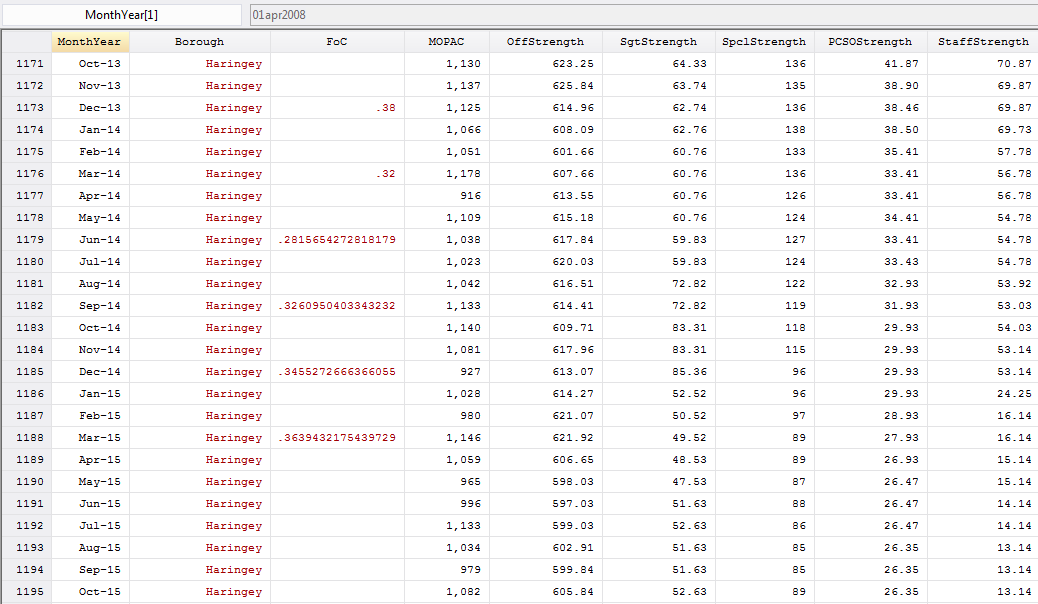
\includegraphics[width=5in]{data2.PNG}

\end{frame}

\begin{frame}
  \frametitle{Example 1}
  \framesubtitle{Cleaning Data}
The reason why Stata thinks our fear of crime variable is a string is that some of the values have \% characters (probably an artefact of inconsistent Excel cell formatting).

\smallskip

We can remove these using the -subinstr- command

\lstinputlisting[linerange={lstart-lend}]{../../stata/logs/destring.log}
\end{frame}


%% Remove?
\begin{frame}
  \frametitle{Example 1}
  \framesubtitle{Cleaning Data}
We also need to encode a numerical version of our Borough variable in order to finish setting up the data 

\lstinputlisting[linerange={lstart-lend}]{../../stata/logs/encode.log}

\end{frame}

%%%%%%%%%%%%%%%%%%%%%%%%%%%%%%%

\begin{frame}
  \frametitle{Presenting Results with Stata}
  \framesubtitle{Tables}
The -estout- program is a good way to present professional looking regression tables.

\medskip

You usually want to present the results of several models side by side
  \begin{itemize}
    \item After each regression, save the results of the model using -eststo-
    \item Create a table using -esttab-
    \item You can save the table as an rtf file, and include a link to it in a word document that can be refreshed if you change your analysis
  \end{itemize}
\end{frame}



\begin{frame}
  \frametitle{Presenting Results with Stata}
  \framesubtitle{Regression results}

\begin{columns}[onlytextwidth]
  \begin{column}{6cm}

\lstinputlisting[linerange={lstart-lend}]{../../stata/logs/esttab.log}
\normalsize

  \end{column}
  \begin{column}{6cm}
{
\def\sym#1{\ifmmode^{#1}\else\(^{#1}\)\fi}
\begin{tabular}{l*{2}{c}}
\hline\hline
            &\multicolumn{1}{c}{(1)}&\multicolumn{1}{c}{(2)}\\
            &\multicolumn{1}{c}{price}&\multicolumn{1}{c}{price}\\
\hline
mpg         &      -238.9\sym{***}&      -271.6\sym{***}\\
            &     (-4.50)         &     (-4.70)         \\
[1em]
rep78       &                     &       667.0         \\
            &                     &      (1.95)         \\
[1em]
\_cons      &     11253.1\sym{***}&      9657.8\sym{***}\\
            &      (9.61)         &      (7.17)         \\
\hline
\(N\)       &          74         &          69         \\
\hline\hline
\multicolumn{3}{l}{\footnotesize \textit{t} statistics in parentheses}\\
\multicolumn{3}{l}{\footnotesize \sym{*} \(p<0.05\), \sym{**} \(p<0.01\), \sym{***} \(p<0.001\)}\\
\end{tabular}
}

  \end{column}
\end{columns}

\end{frame}


\begin{frame}
  \frametitle{Presenting Results with Stata}
  \framesubtitle{Regression results}
After running a regression, you can access post-estimation statistics with -ereturn-.

\lstinputlisting[linerange={lstart-lend}]{../../stata/logs/post.log}

\end{frame}



\begin{frame}
  \frametitle{Presenting Results with Stata}
  \framesubtitle{Regression results}
You can access these and use them just like any other number with e([statistic])

\lstinputlisting[linerange={lstart-lend}]{../../stata/logs/post_r2.log}

\end{frame}

\begin{frame}
  \frametitle{Presenting Results with Stata}
  \framesubtitle{Regression results}
You can also view a matrix of the coefficients

\lstinputlisting[linerange={lstart-lend}]{../../stata/logs/post_mb.log}

\end{frame}

\begin{frame}
  \frametitle{Presenting Results with Stata}
  \framesubtitle{Regression results}
And the variance covariance matrix

\lstinputlisting[linerange={lstart-lend}]{../../stata/logs/post_mv.log}

\end{frame}

\begin{frame}
  \frametitle{Presenting Results with Stata}
  \framesubtitle{Regression results}
As well as individual coefficients and standard errors
\lstinputlisting[linerange={lstart-lend}]{../../stata/logs/post_ib.log}

\end{frame}



\begin{frame}
  \frametitle{Presenting Results with Stata}
  \framesubtitle{Regression results}

\begin{columns}[onlytextwidth]
  \begin{column}{5.5cm}
This is useful because we can specify the statistics we want to include in our regression table with the stats option.
\lstinputlisting[linerange={lstart-lend}]{../../stata/logs/esttab_2.log}
\normalsize

  \end{column}
  \begin{column}{6cm}

{
\def\sym#1{\ifmmode^{#1}\else\(^{#1}\)\fi}
\begin{tabular}{l*{2}{c}}
\hline\hline
            &\multicolumn{1}{c}{(1)}&\multicolumn{1}{c}{(2)}\\
            &\multicolumn{1}{c}{price}&\multicolumn{1}{c}{price}\\
\hline
mpg         &      -238.9\sym{***}&      -271.6\sym{***}\\
            &     (-4.50)         &     (-4.70)         \\
[1em]
rep78       &                     &       667.0         \\
            &                     &      (1.95)         \\
[1em]
\_cons      &     11253.1\sym{***}&      9657.8\sym{***}\\
            &      (9.61)         &      (7.17)         \\
\hline
N           &          74         &          69         \\
r2          &       0.220         &       0.251         \\
F           &       20.26         &       11.06         \\
\hline\hline
\multicolumn{3}{l}{\footnotesize \textit{t} statistics in parentheses}\\
\multicolumn{3}{l}{\footnotesize \sym{*} \(p<0.05\), \sym{**} \(p<0.01\), \sym{***} \(p<0.001\)}\\
\end{tabular}
}


  \end{column}
\end{columns}

\end{frame}

\begin{frame}
  \frametitle{Presenting Results with Stata}
  \framesubtitle{Regression results}

\begin{columns}[onlytextwidth]
  \begin{column}{5.5cm}
We can also calculate our own statistics, and include them in the model. Here we compute the turning point for a squared term
\lstinputlisting[linerange={lstart-lend}]{../../stata/logs/esttab_tp.log}
\normalsize

  \end{column}
  \begin{column}{6cm}

{
\def\sym#1{\ifmmode^{#1}\else\(^{#1}\)\fi}
\begin{tabular}{l*{2}{c}}
\hline\hline
            &\multicolumn{1}{c}{(1)}&\multicolumn{1}{c}{(2)}\\
            &\multicolumn{1}{c}{price}&\multicolumn{1}{c}{price}\\
\hline
weight      &      -7.273\sym{**} &      -9.040\sym{**} \\
            &     (-2.70)         &     (-3.11)         \\
[1em]
sqweight    &     0.00151\sym{***}&     0.00168\sym{***}\\
            &      (3.49)         &      (3.79)         \\
[1em]
mpg         &                     &      -124.8         \\
            &                     &     (-1.53)         \\
[1em]
\_cons      &     13418.8\sym{**} &     19804.8\sym{***}\\
            &      (3.36)         &      (3.44)         \\
\hline
tp          &      2401.7         &      2691.3         \\
\hline\hline
\multicolumn{3}{l}{\footnotesize \textit{t} statistics in parentheses}\\
\multicolumn{3}{l}{\footnotesize \sym{*} \(p<0.05\), \sym{**} \(p<0.01\), \sym{***} \(p<0.001\)}\\
\end{tabular}
}


  \end{column}
\end{columns}

\end{frame}



\begin{frame}
  \frametitle{Presenting Results with Stata}
  \framesubtitle{Graphs}
-graph twoway- has many different ways to show relationships between variables
\begin{columns}[onlytextwidth]
  \begin{column}{5.5cm}
Here we show a basic scatter plot
\Tiny
\lstinputlisting[linerange={lstart-lend}]{../../stata/logs/graph_scatter.log}
\normalsize
After saving, we can insert a picture as link into word
  \end{column}
  \begin{column}{6cm}
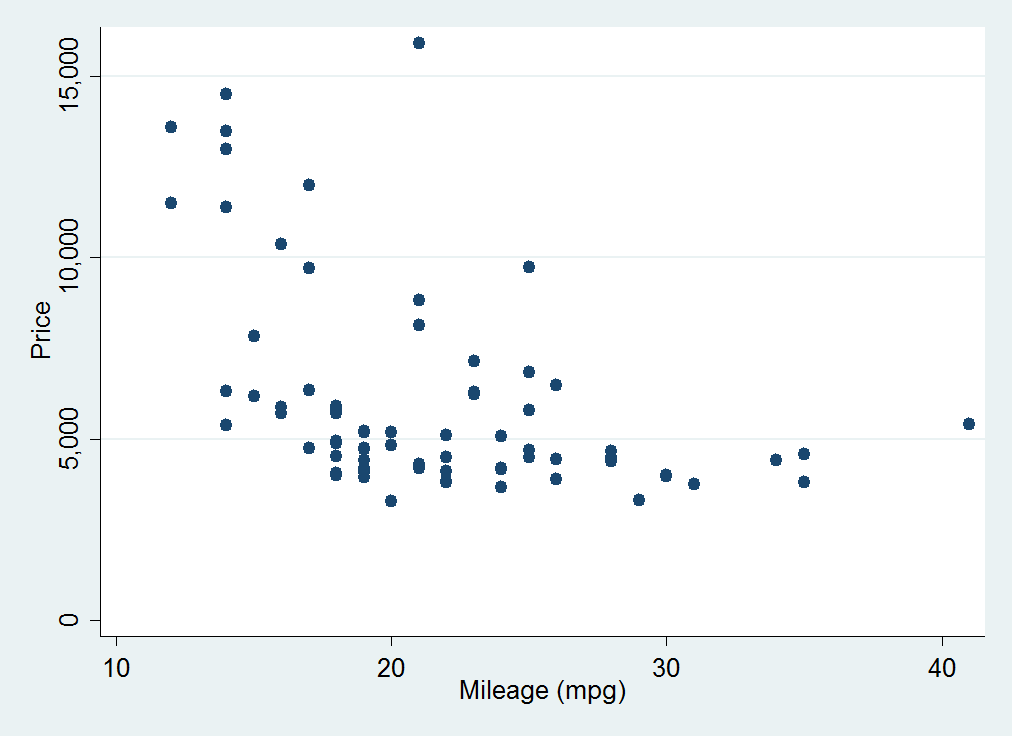
\includegraphics[width=2.5in]{../../word/scatter.PNG}
  \end{column}
\end{columns}

\end{frame}



\begin{frame}
  \frametitle{Presenting Results with Stata}
  \framesubtitle{Graphs}
-twoway- is extendable - we can overlay lots of plots one on top of the other
\begin{columns}[onlytextwidth]
  \begin{column}{5.5cm}
We just add each plot in a set of brackets
\lstinputlisting[linerange={lstart-lend}]{../../stata/logs/graph_overlay.log}
  \end{column}
  \begin{column}{6cm}
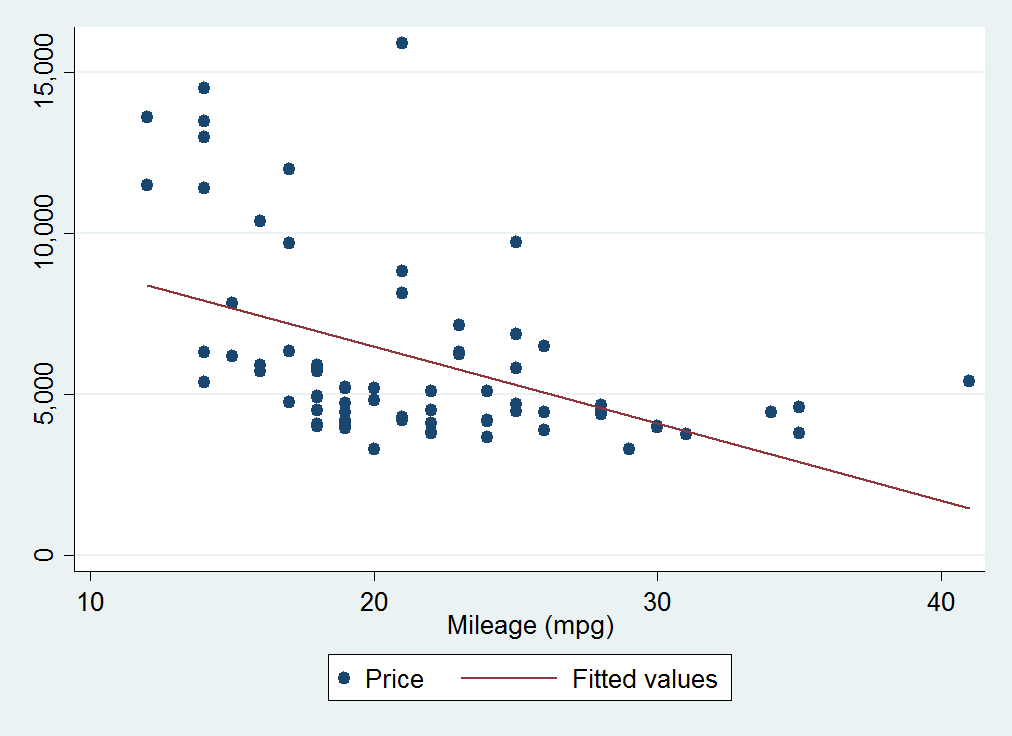
\includegraphics[width=2.5in]{../../word/overlay.PNG}
  \end{column}
\end{columns}

\end{frame}

\begin{frame}
  \frametitle{Presenting Results with Stata}
  \framesubtitle{Graphs}
Various schemes are available -  a lighter option than built schemes can be downloaded with -ssc install burd-
\begin{columns}[onlytextwidth]
  \begin{column}{5.5cm}
\lstinputlisting[linerange={lstart-lend}]{../../stata/logs/scheme.log}
  \end{column}
  \begin{column}{6cm}
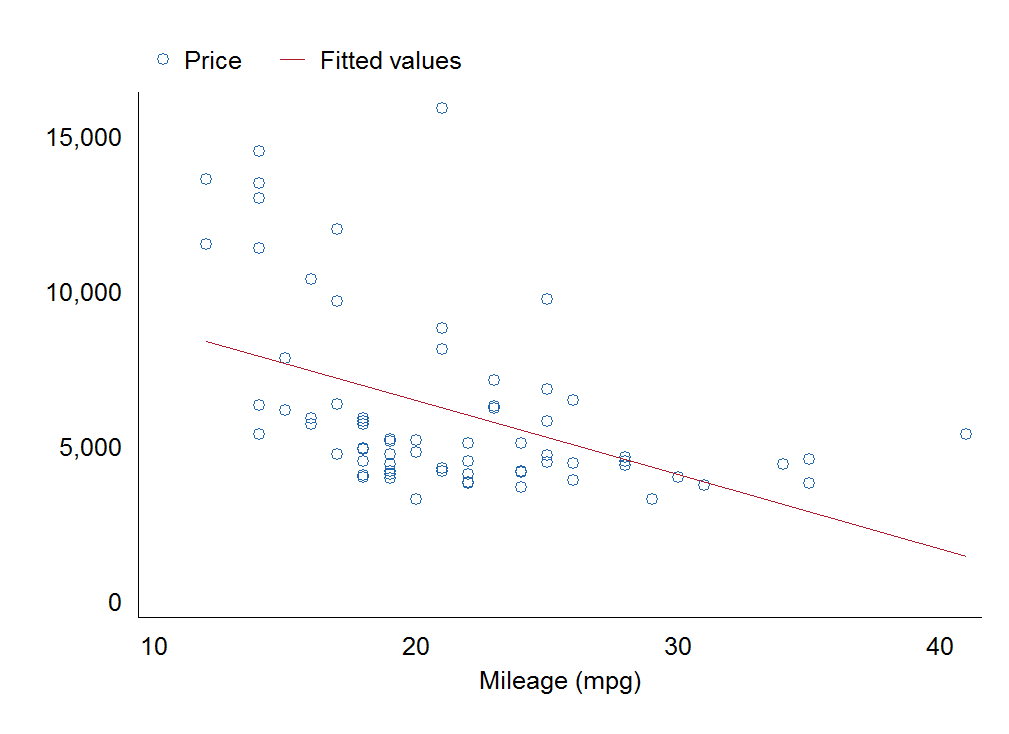
\includegraphics[width=2.5in]{../../word/scheme.PNG}
  \end{column}
\end{columns}

\end{frame}


\begin{frame}
  \frametitle{Presenting Results with Stata}
  \framesubtitle{Graphs}
There are many more options we can set for the graph. They can be applied universally, or to individual layers
\begin{columns}[onlytextwidth]
  \begin{column}{5.5cm}
\lstinputlisting[linerange={lstart-lend}]{../../stata/logs/graph_options.log}
  \end{column}
  \begin{column}{6cm}
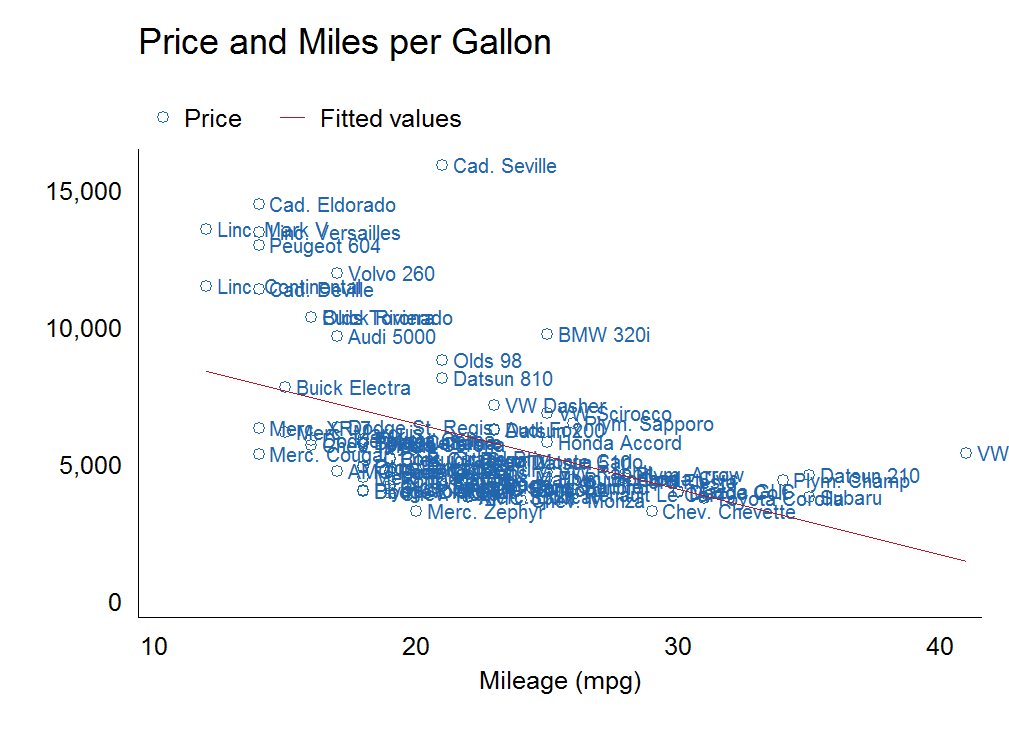
\includegraphics[width=2.5in]{../../word/graph_options.PNG}
  \end{column}
\end{columns}

\end{frame}


\begin{frame}
  \frametitle{Presenting Results with Stata}
  \framesubtitle{Graphs}
-graph matrix- draws a scatterplot matrix showing the relationship between pairs of variables in a list

\medskip

You can apply it to all numeric variables
  \begin{itemize}
    \item 
  \end{itemize}
\end{frame}



\begin{frame}
  \frametitle{Presenting Results with Stata}
  \framesubtitle{Graphs}
-graph matrix-
  \begin{itemize}
    \item 
  \end{itemize}
\end{frame}

\begin{frame}
  \frametitle{References}
\bibliography{stata.bib}
\bibliographystyle{plain}
\end{frame}


\end{document}